\paragraph{MAKG} \mbox{}

Michael Färber has processed the data from the papers and offers dump files in \acrfull{rdf} format \cite{faerber2019microsoft} and also provides an SPARQL endpoint\footnote{\url{https://makg.org/sparql}}. Each file includes different information, such as metadata about the subjects, the authors or the papers. The abstracts have also been reconstructed into free text, as Microsoft only provides them as lists of tokens.

Färber's dumps comprise over 238 million publications and 740,460 subjects\footnote{These numbers refer to the dump of 29.05.2020}. How the subjects are distributed among the fields (i.e. the subjects of the first level) is displayed in figure \ref{fig:subjects_per_field_per_level}. This plot only considers the subjects that are part of the hierarchy. There are 196,631 subjects (27 \%) that do not belong to any of the fields.

341,959 subjects of the hierarchy (46 \%) belong to the fields of biology and medicine. Environmental science is the least represented field, with only 126 subjects, followed by history, which comprises 1,510 subjects. Regarding the levels, there are 19 subjects in the first level (called fields from now on) and 292 in the second. The latter ones include over 100,000 subjects per level, incrementally increasing and peaking at 165,321 subjects in the sixth level.

\begin{figure}
    \centering
    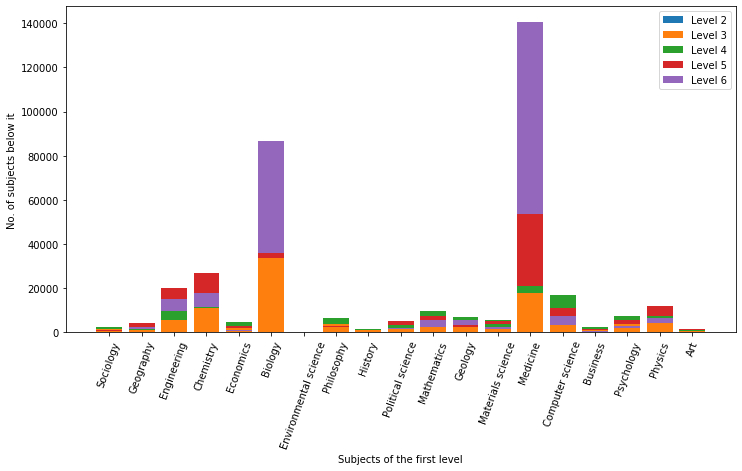
\includegraphics[width=\textwidth]{figures/related_work/makg/subjects_per_field_per_level.png}
    \caption{Subjects present in the MAKG.}
    \label{fig:subjects_per_field_per_level}
\end{figure}

\begin{figure}
    \centering
    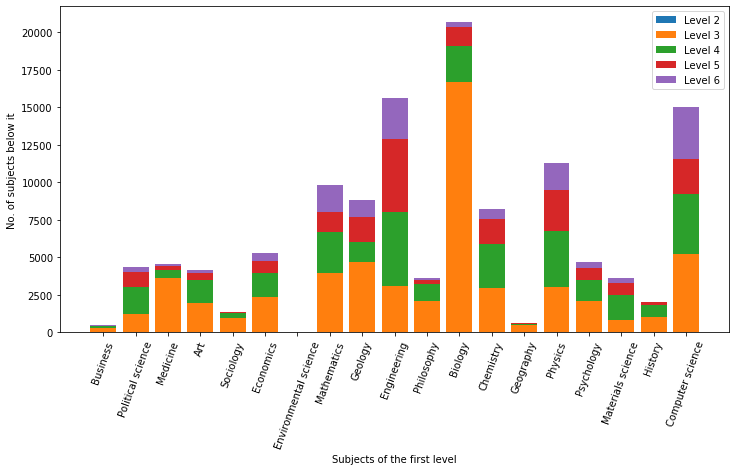
\includegraphics[width=\textwidth]{figures/related_work/makg/subjects_w_article.png}
    \caption{Subjects of the MAKG that have a Wikipedia link.}
    \label{fig:subjects_w_article}
\end{figure}

\begin{figure}
    \centering
    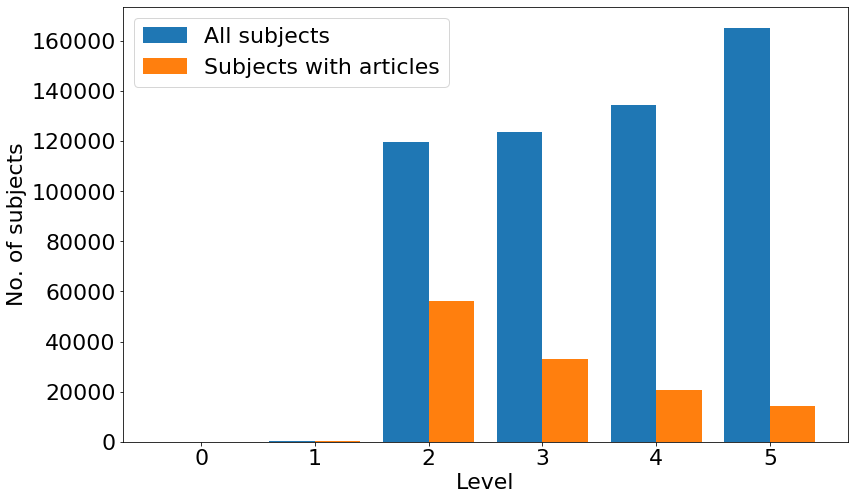
\includegraphics[width=.75\textwidth]{figures/related_work/makg/subject_distribution_comparison.png}
    \caption{Comparison of all subjects with the subset that have a Wikipedia link.}
    \label{fig:subject_distribution_comparison}
\end{figure}

124,385 subjects (17 \% of all subjects) have a Wikipedia link. These are shown in figure \ref{fig:subjects_w_article}. They are relevant for computing the vector representations of the subjects. If they are not present, we cannot do so, as we don't have a text associated to the subject we can use for the vectorization procedure. Biology is the field with the most links, followed by Computer Science and Engineering. Only 4,574 subjects of the 179,741 in the field of Medicine (2.5 \%) have a link, which is why this field is no longer the most populated field when considering Wikipedia links. The difference among all subjects and those with links is shown in figure \ref{fig:subject_distribution_comparison} on a per-level basis. When looking at all subjects, the number increases with the level. When looking at the subjects with links, the opposite occurs: the number of subject decreases with the level.

Regarding the subject assignments of the documents, Färbers files don't include all the subjects assigned to each document. When querying the SPARQL endpoint for all subjects that have been assigned to at least one paper, only 19 subjects are returned. They are very broad subjects, such as \textit{Geology} or \textit{Computer Science}. The assigned subjects in Färbers \acrshort{rdf} files also don't always coincide with the ones assigned by Microsoft. For example, in the \acrshort{rdf} files the paper \textit{Determination of vitamin D3 and 25-hydroxyvitamin D3 in foodstuffs by HPLC UV-DAD and LC–MS/MS} has the subject \textit{Environmental Science}, whereas in Microsoft Academic the topics assigned to the publication include \textit{Vitamin}, \textit{High-performance liquid chromatography} and eight others. These subjects can be retrieved through the \acrshort{api}.